\ifdefined\XeTeXversion\else\pdfoutput=1\fi
\documentclass[11pt]{article}

\usepackage[margin=1.15in]{geometry}
\usepackage{amsmath}
\usepackage{mathptmx}
\usepackage{graphicx}
\usepackage{booktabs}
\usepackage{microtype}
\usepackage[hidelinks]{hyperref}
\usepackage{url}
\urlstyle{same}

\title{Memory Is the Price: Evidence from the LLM Serving Market on the
Economics of Mixture-of-Experts Inference}

\author{Michael J.\ Yuan, PhD\thanks{ByteFuture Inc.} \and Ju Long, PhD\thanks{Texas State University}}

\date{Working paper $\cdot$ Draft of July 2026\\\small Data collected 2026-07-06}

\begin{document}
\maketitle

\begin{abstract}
Sparse Mixture-of-Experts (MoE) models are widely claimed to cost what their
\emph{active} compute costs. We test this claim against the LLM serving
market itself. Because providers disclose almost nothing about their
production systems, we treat posted prices as an observable proxy for the
latent serving configuration. From OpenRouter's public endpoints API we
assemble a snapshot (2026-07-06) of every open-weight, general-purpose model
served by at least three providers: 46 models, of which 38 form the primary
panel of 289 provider--model observations from 42 providers, with
architecture verified against each model's HuggingFace repository. The
DeepSeek panels are excluded from the primary specification because the
vendor anchors its own serving prices, and are analyzed separately. The
prices contradict the compute-pricing claim. A hedonic log-log regression of
median output price on active parameters and the sparsity ratio yields a
sparsity elasticity of 0.481 ($t = 4.9$, $p = 1.9 \times 10^{-5}$), 84\% of
the active-parameter elasticity; the regression is jointly significant with
$F(2,35) = 16.8$ ($p = 7.7 \times 10^{-6}$) and $R^2 = 0.49$. MoE models are
therefore billed most of the way toward their total memory footprint, and
customers keep little of the advertised compute discount. Market structure
supports the scale interpretation in part. The price floor of every panel of
200B+ total parameters belongs to a vertically integrated provider, a
neocloud in eleven of seventeen panels and the model's own vendor in six.
Hyperscalers price 1.2--8.8$\times$ above the floor and never set it.
Participation, however, no longer declines with model size: trillion-scale
panels now attract 11--22 providers, consistent with the diffusion of
published expert-parallel serving recipes. MoE price dispersion remains
compressed relative to dense models (median coefficient of variation 0.23
versus 0.35). DeepSeek is the revealing exception: its sparse-attention
generation is served at roughly one fifth of the schedule price, and the
vendor itself sets the floor beneath its flagship, which is the
vertical-integration mechanism in its purest form.
\end{abstract}

\section{Introduction}

Between 2024 and 2026, the architecture of frontier open-weight language
models changed decisively. Mixtral 8x7B (December 2023) reintroduced the
sparse Mixture-of-Experts (MoE) design to open models with 8 experts per
layer, of which 2 are activated per token. DeepSeek-V3 and R1 (December 2024 /
January 2025) scaled the recipe to 671 billion total parameters with only 37
billion active per token (256 routed experts, top-8 routing)~\cite{r15}.
Within eighteen months, essentially every major open-weight release followed:
Llama 4 Scout and Maverick (16 and 128 experts,
top-1)~\cite{hf_scout,hf_maverick}, Qwen3-235B (128 experts,
top-8)~\cite{hf_qwen}, Kimi K2 (one trillion parameters, 384
experts)~\cite{hf_kimi}, GPT-OSS-120B (128 experts, top-4)~\cite{hf_oss},
GLM-4.5 (160 experts)~\cite{hf_glm}, and MiniMax M2 (256
experts)~\cite{hf_minimax}. The sparsity ratio (total to active parameters) has grown
from $\sim$4$\times$ in Mixtral to 18--31$\times$ in the current frontier.
Meanwhile the largest open \emph{dense} models have retreated: Llama-3.1-405B,
the largest dense open release, is effectively delisted from the commercial
serving market as of mid-2026.

Sparsity is marketed as an efficiency technology. The paper that popularized
the design promised ``outrageous numbers of parameters'' at ``a constant computational cost''~\cite{r30}, and on compute-based reasoning a
671B-parameter model that computes with only 37B parameters per token should
cost about as much to serve as a 37B dense model~\cite{r31,r32}. Market prices
do not bear this out. At the time of our data collection, Kimi K2.6 (one
trillion total parameters, 32B active) commanded a median output price of
\$3.55 per million tokens across twenty providers, while Llama-3.3-70B, a
dense model with more than twice K2.6's active parameters, cost \$0.72. Per
unit of active compute, the MoE model is roughly eleven times more
expensive. A second irregularity compounds the first: prices for the
\emph{same} model differ substantially across providers. Google lists
Qwen3-235B-A22B at \$0.88 per million output tokens while DeepInfra lists it
at \$0.10, a spread of nearly nine times on identical weights.

These patterns cannot be explained from provider disclosures, because there
are almost none. The production systems behind commercial inference endpoints
are, with rare exceptions, undisclosed. Hyperscaler model catalogs publish
prices, context windows, regions, and quotas, but not hardware, served
precision, parallelism, or cluster scale; Google's managed-Llama announcement
states simply that ``the underlying infrastructure, scaling, and management
costs are incorporated into the API usage price''~\cite{r25}. On OpenRouter,
the marketplace whose data we use, the per-endpoint schema contains no field
for hardware or deployment topology, and even the self-reported quantization
tag is frequently ``unknown''~\cite{r1}. The opacity extends to the served
model itself: a black-box audit found that 11 of 31 commercial Llama endpoints
produced output distributions deviating from Meta's reference weights, because
providers ``may quantize, watermark, or finetune the underlying
model\ldots\ possibly without notifying users''~\cite{r23}.

The secrecy is not uniform, and the exceptions delimit what is actually
hidden. The serving software stack is open source (vLLM, SGLang), and the techniques for efficient MoE serving are published. DeepSeek, a model vendor with an evident strategic interest in commoditizing the serving of its own models, has disclosed its production system in detail, down to its EP144 decode topology and a theoretical 545\% margin~\cite{r10}. Third parties have publicly reproduced that recipe~\cite{r8}. What remains hidden is the mapping
from any \emph{particular} commercial endpoint to its deployment: which
provider runs expert parallelism at what scale, at what batch size and
utilization, at what unit cost. Engineering blogs occasionally reveal
fragments (Cloudflare, for instance, has described the multi-node system
behind its largest models~\cite{r19}), but for the 42 providers in our
panel, the economically decisive parameters are unobservable.

The one thing every provider must publish is a price. This turns an
information-asymmetry problem into an inference problem with a classical
structure. The serving configuration behind an endpoint (cluster scale,
parallelism degree, batch size, served precision, utilization) is the
provider's private information; the observer sees only the posted price. But prices are the market's mechanism for aggregating dispersed private information~\cite{r26}. Open-weight serving, moreover, approximates the textbook competitive case: the weights are free, the software is open source, entry is
unrestricted, and dozens of providers quote side by side on a public
marketplace. Competition disciplines posted prices toward marginal cost, and
marginal cost is a function of the serving technology chosen. Sustained price
structure therefore serves as an observable proxy for the latent cost
structure and, through it, for the latent hardware configuration that
generates that cost structure. Our empirical strategy follows the
hedonic-pricing tradition~\cite{r27}: we regress prices on the product
characteristics that drive resource consumption (active parameters; total
memory footprint) and read the estimated coefficients as implicit prices, the
market's marginal valuation of each underlying resource. The industry's claim
that sparsity's compute savings pass through into proportionally cheaper
serving then becomes a testable restriction on hedonic coefficients (H1). The question of what serving scale is required to capture those savings becomes a prediction about which provider class posts each panel's price floor, who participates in each market, and how endogenous participation truncates the observed price distribution (H2).

We are explicit about the limits of this inversion. Price is a low-dimensional
proxy: it cannot reconstruct any single endpoint's configuration, and an
individual quote confounds cost with strategy (loss leaders, price
discrimination, enterprise positioning). Our inferences accordingly rest on
moments of the price distribution that are difficult to generate
strategically: elasticities estimated across 38 models, price floors
replicated across seventeen independent panels, and participation patterns
across 42 providers.

Three strands of prior work frame our contribution. Bottom-up cost models
compute what MoE serving \emph{should} cost under optimal
deployment~\cite{r24,r7} but do not test market prices. Black-box measurement studies characterize hosted endpoints behaviorally. Gao et al.\ detect undisclosed weight modifications from outputs~\cite{r23}. Li et al.\ document that hosted open-weight APIs are heterogeneous services whose listed prices are their most anchored attribute, observing descriptively, without a regression, that neither total nor active parameter count suffices to explain price~\cite{r22}. Closest to our first hypothesis, Scher compared five MoE
models against a dense price trendline in early 2025 and observed informally
that MoE prices sit ``somewhere between their active and total parameter
count, perhaps closer to the total parameter count''~\cite{r21}. We formalize
that observation into an identified quantity. To our knowledge, this paper
makes three contributions. It provides the first hedonic estimate of the sparsity elasticity of price (\S\ref{sec:h1result}). It presents the first evidence that the price floors for large MoE models are set exclusively by massively parallel providers (\S\ref{sec:h2result}). And it provides the first documentation that provider participation, and through selection the measured price dispersion, is gated by model memory footprint (\S\ref{sec:h2result}--\ref{sec:dispersion}). The concluding section draws out
the hardware implication.

\section{Background and hypotheses}

\subsection{Background: the cost structure of decoding}
\label{sec:background}

Transformer inference has two phases. \emph{Prefill} processes the prompt in
parallel and is compute-bound. \emph{Decode} generates output tokens one at a
time; each step must read the model's weights from memory while performing
only $\sim$2 floating-point operations per parameter read, making it
memory-bound on all practical hardware. Output-token prices therefore reflect
decode economics, and we study output prices throughout.

Two facts about the input markets frame our hypotheses. First, high-bandwidth memory (HBM) is the expensive and supply-constrained component of AI accelerators. HBM3E commanded a price premium more than four times that of DDR5 in 2025~\cite{r4} and represents roughly 40--50\% of an accelerator's manufacturing cost~\cite{r5}. SK hynix, the leading supplier, sold out its capacity into 2026~\cite{r6}. Second, the number of GPUs a provider must deploy for a model is determined by the model's \emph{total} memory footprint, not by its compute. DeepSeek R1 at FP8 requires $\sim$700 GB for weights, making an 8$\times$H200 node (1{,}128 GB) the standard minimal deployment~\cite{r17}; Kimi K2 at FP8 fills the same node almost completely.
Sparsity does not reduce this footprint: although only $k$ of $E$ experts fire
per token, all $E$ must reside in memory, because different tokens in a batch
activate different experts~\cite{r7}.

A third fact concerns serving efficiency at scale. On a single 8-GPU node, a
256-expert model cannot be batched to compute efficiency. With top-8 routing, each expert receives only $K/32$ tokens per step from a batch of $K$, far below the $\sim$128-token tile that saturates the grouped-GEMM kernels. The node therefore remains memory-bound at well under 1\% model-FLOPS utilization at any feasible batch~\cite{r9,r16}. Recovering efficiency requires \emph{expert
parallelism} (EP): spreading experts across many GPUs and aggregating tokens
from thousands of concurrent users so that every expert sees full tiles.
Published EP deployments include SGLang's 96$\times$H100 system~\cite{r8} and
DeepSeek's own production units of EP144 across 18 nodes~\cite{r10}.

\subsection{Hypothesis 1: sparsity makes inference cheap (the compute-pricing view)}
\label{sec:h1}

The proposition that MoE reduces serving cost by reducing compute has
accompanied the architecture since its introduction, stated by its strongest
proponents. Switch Transformers promised models ``with outrageous numbers of parameters'' at ``a constant computational cost''~\cite{r30}. Mistral's
Mixtral 8x7B announcement drew the pricing implication explicitly: the model
``only uses 12.9B parameters per token'' and ``therefore, processes input and
generates output at the same speed and for the same cost as a 12.9B
model''~\cite{r31}. Databricks made the same argument for DBRX, crediting
``about half as many active parameters'' for inference ``up to 2x faster than
LLaMA2-70B''~\cite{r32}. Taken at face value, the claim yields a sharp
prediction about market prices: a model's output price is determined by its
active parameters, and the sparsity ratio is free to the customer. We adopt
this prediction as our first hypothesis. Formally, in the hedonic price
regression
\begin{equation}
\log(\text{price}) = c_0 + c_1 \log(\text{active\_params})
                        + c_2 \log(\text{total}/\text{active})
\label{eq:hedonic}
\end{equation}
the coefficients are implicit prices in Rosen's sense~\cite{r27}. The coefficient $c_1$ is the market's marginal valuation of active compute, and $c_2$ is its valuation of resident-but-inactive parameters, the capacity that must be held in memory although it does not fire. \emph{H1 (compute pricing)} predicts $c_2 = 0$. The
alternative follows from \S\ref{sec:background}. If memory rather than compute is the first-order cost of serving, because capital tied up in HBM scales with bytes held and decode throughput is limited by bytes streamed, then prices should track the \emph{total} footprint. This implies $c_2 \approx c_1$: a 671B/37B MoE is billed like a 671B dense model. The ratio $c_2/c_1$ therefore measures the
share of the advertised sparsity discount that the market withholds from
customers. Under H1 the ratio is zero, because the full compute saving
passes through to prices; under the memory-pricing alternative it approaches
one, and customers keep none of the discount.

\subsection{Hypothesis 2: capturing the compute savings requires scale}
\label{sec:h2}

While H1 concerns the composition of serving cost (which resource the market
prices), our second hypothesis concerns scale economies: the minimum efficient
scale at which a provider can realize the compute savings of sparsity. The
mechanism of \S\ref{sec:background} implies that these savings, whatever share
of them reaches customers, are only captured when enough concurrent traffic is
aggregated that every expert sees full tiles, and that requires dedicated,
disaggregated decoding infrastructure far larger than a single node. The serving-systems literature
has converged on exactly this design. Splitwise showed that splitting the prefill
and decode phases onto separate machine pools yields 1.4$\times$ throughput at
20\% lower cost, observing that the decode phase ``does not require the compute capability of the latest GPUs''~\cite{r33}. DistServe disaggregates the phases onto different GPUs for up to 7.4$\times$ goodput~\cite{r34}. Moonshot's production platform for Kimi, Mooncake, ``separates the prefill and decoding clusters'' outright~\cite{r35}. For large MoE, the decode pool must
additionally be expert-parallel, spread across tens to hundreds of
GPUs~\cite{r8,r10,r11}. The economic consequence is H2: the
ability to serve large MoE at competitive prices is confined to providers who
operate such pools and can amortize them across massive request volume. This
predicts three observable market patterns. (a) The \emph{price floor} for each large-MoE model should be set by specialized high-volume GPU clouds (``neoclouds'') rather than by general-purpose clouds. (b) General-purpose clouds, whose business does not justify dedicated EP pools per open model, should price visibly above the floor. (c) Providers that cannot justify EP infrastructure at all (edge networks, boutique hosts, and by extension on-premises operators) should not offer large MoE models, exiting rather than listing at uncompetitive prices. A corollary concerns price
\emph{dispersion}: because exit removes the high-cost providers from
observation, the measured spread of prices for large MoE should be
\emph{compressed} relative to dense models that any provider can serve.

\section{Method and data}

\subsection{Price panel}

We collected the complete endpoint listings for open-weight models from
OpenRouter's public endpoints API on 2026-07-06, the data source underlying
its public model pages~\cite{r1,r2}. The candidate universe is mechanical
rather than curated: every model listed with a HuggingFace weights
repository qualifies as a candidate, excluding code-specialized models,
vision-language variants, community merges, and alias listings that point to
the same weights as a versioned listing. This yields 129 candidate models
and 532 raw endpoint rows. We excluded free tiers, zero-price rows, and
deranked or offline endpoints. The unit of observation is one quote per
provider per model; where a provider lists multiple endpoints for the same
model, the cheapest is kept, which is the price a customer comparing
providers would face. Models with fewer than three qualifying providers were
then dropped, and the panel values were spot-verified against provider
price pages (\S\ref{sec:verify}). The result is 46 qualifying panels comprising 347
provider--model observations.

The primary specification excludes the seven DeepSeek panels. The exclusion
is on identifying-assumption grounds stated in \S\ref{sec:methods}, not on
fit. DeepSeek is the one vendor that both anchors the market price of its
own models and publishes its serving stack to third parties. Its panels
therefore do not measure the competitive third-party serving process that
identifies cost structure. Section~\ref{sec:deepseek} analyzes the DeepSeek panels
against the schedule estimated without them. The primary panel is
\textbf{38 models (28 MoE spanning expert-to-activation ratios $E/k$ from 4
to 128, and 10 dense) comprising 289 observations from 42 distinct
providers}.

\subsection{Architecture data}

For each model we recorded total parameters, active parameters per token,
expert count $E$, and routing top-$k$, verified against the model
repository's HuggingFace \path{config.json} and model card (fetched at
collection time)~\cite{hf_scout,hf_maverick,hf_qwen,hf_kimi,hf_oss,hf_glm,hf_minimax,hf_r1}.
The archived architecture file records the repository for every panel model.
Two verification notes apply. First, safetensors parameter counts are
unreliable for quantization-packed checkpoints, so official model-card
figures take precedence; DeepSeek V4 Flash, for example, is 284B total
parameters by its card although its packed checkpoint stores fewer tensor
elements. Second, MiniMax M3 does not publish its expert count, so it is
excluded from the analyses that require $E/k$. Dense models take active =
total and $E/k = 1$.

\subsection{Verification pass}
\label{sec:verify}

Two mechanical rules produce the final panel from the raw rows, and both are
checkable against the archived data: the one-quote-per-provider rule and the
three-provider threshold stated above. In addition, the panel's single most
extreme value, DeepInfra's \$0.10/M output price on Qwen3-235B-A22B, roughly
eight times below its panel median, was confirmed on DeepInfra's own price
page~\cite{r18}. Quantization does not explain the widest within-model
spreads: in the widest panels the minimum and maximum prices are posted at
comparable quantizations, and the largest spreads separate neocloud
listings from hyperscaler managed offerings.

\subsection{Statistical methods}
\label{sec:methods}

To test H1 we compute each model's median output price across providers
(robust to loss-leaders and premium listings) and fit the hedonic
regression~\eqref{eq:hedonic} by ordinary least squares ($n = 38$). The
identifying assumption is that competing third parties' posted prices reveal
the cost structure of serving. This assumption fails for DeepSeek: the
vendor lists its own models at strategically chosen prices, publicly commits
to commoditizing the serving of its own models, and publishes its serving
recipes~\cite{r10,r8}, so third-party quotes for DeepSeek models are
anchored rather than competitive. We therefore estimate the schedule without
the DeepSeek panels. Three robustness variants are reported: the full
46-model universe, the panel with every vendor's own endpoints removed
(which shows the exclusion is not doing hidden work), and the DeepSeek
panels evaluated against the primary schedule (\S\ref{sec:deepseek}). We report standard
errors, $t$-statistics, and $p$-values for every coefficient, and the
regression $F$-statistic. To test H2 (\S\ref{sec:h2}) we proceed as before:
we identify each panel's floor-setting provider and its class, compare
hyperscaler listings with panel floors, relate provider participation to
model footprint, and measure within-model dispersion for MoE versus dense
panels. All statistics are computed deterministically from the archived
JSON by \path{analysis.py}, with no model-generated numbers.

\section{Results}

\subsection{H1 rejected: the market prices memory footprint, not active compute}
\label{sec:h1result}

Figure~\ref{fig:level} plots median output price against active parameters
on log-log axes. The ten dense models trace a price line with a slope near
unit elasticity ($\log_{10} p = -1.691 + 0.950\,\log_{10}(\text{active})$).
Every MoE model sits above it, by 1.0$\times$ to 21.6$\times$ with a median
of 5.0$\times$, and the excess grows with the model's sparsity ratio.

\begin{figure}[t]
\centering
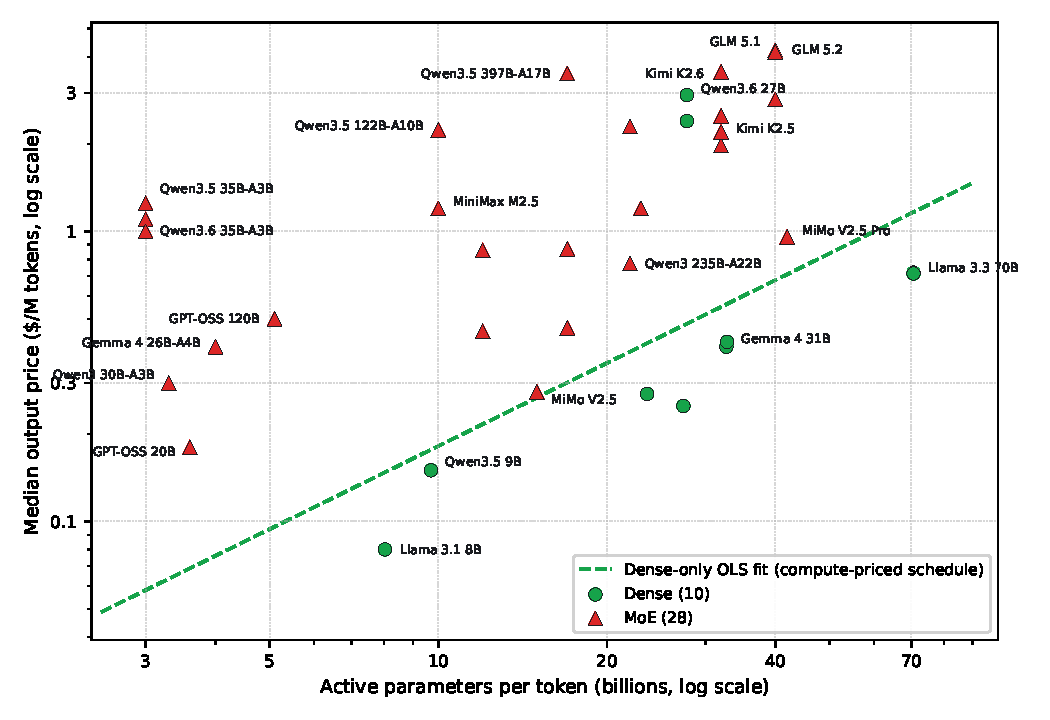
\includegraphics[width=\linewidth]{fig1_price_level.pdf}
\caption{The figure plots median output price against active parameters per
token for the 38 primary-panel models on log-log axes, with dense models as
green circles and MoE models as red triangles; selected models are labeled.
The dashed line is the dense-only OLS fit, which is the price schedule a
compute-priced market would apply. Every MoE model sits on or above the
line, and the median MoE model sits 5$\times$ above it.}
\label{fig:level}
\end{figure}

The regression quantifies the pattern (Table~\ref{tab:ols}) and rejects H1
(\S\ref{sec:h1}) decisively. Compute pricing predicts $c_2 = 0$; the estimate is 0.481 with
$t = 4.9$ and $p = 1.9 \times 10^{-5}$. The regression is jointly
significant, with $F(2,35) = 16.8$ and $p = 7.7 \times 10^{-6}$, and
explains about half of the variance in log prices ($R^2 = 0.49$). The
sparsity-ratio elasticity is 84\% of the active-parameter elasticity:
$c_2/c_1 = 0.84$. The sparsity ratio, which H1 predicts to be free, is in
fact priced at 84\% of the rate of active compute. The market bills MoE
models most of the way toward their total memory footprint, so a
1{,}000B-total/32B-active model such as Kimi K2.6 is billed roughly like a
$\sim$580B dense model rather than the 32B model its compute would suggest.

The result is robust to the construction of the panel. Including the
DeepSeek panels moves the ratio to 0.85 ($n = 46$, $c_2 = 0.391$,
$p = 2.0 \times 10^{-4}$, $R^2 = 0.37$). Removing every vendor's own
endpoints from every panel leaves it at 0.84 ($n = 34$, $c_2 = 0.468$,
$p = 1.3 \times 10^{-4}$, $R^2 = 0.47$), which shows that the DeepSeek
exclusion, and owner listings generally, are not driving the estimate.

\begin{table}[t]
\centering
\caption{The table reports OLS estimates of the hedonic
regression~\eqref{eq:hedonic} on the primary panel ($n = 38$ models,
$R^2 = 0.490$, $F(2,35) = 16.8$ with $p = 7.7 \times 10^{-6}$). H1 (compute
pricing) predicts $c_2 = 0$, and pure footprint pricing predicts
$c_2 = c_1$; the measured ratio is $c_2/c_1 = 0.84$.}
\label{tab:ols}
\begin{tabular}{lrrrr}
\toprule
Coefficient & Estimate & Std.\ err. & $t$ & $p$ \\
\midrule
$c_1$: log(active parameters) & $+0.572$ & 0.138 & 4.1 & $2.1 \times 10^{-4}$ \\
$c_2$: log(total/active)      & $+0.481$ & 0.097 & 4.9 & $1.9 \times 10^{-5}$ \\
\bottomrule
\end{tabular}
\end{table}

Table~\ref{tab:panel} reports the underlying panel. Per active parameter,
the MoE models cost up to 40$\times$ more than the dense reference (Qwen3.5
35B-A3B at \$0.42 per active-parameter-billion against $\sim$\$0.010 for the
Llama dense models). The premium over the dense line tracks the sparsity
ratio: the extremely sparse small MoE models (Qwen3.5 and Qwen3.6 35B-A3B,
Qwen3 Next 80B-A3B) sit 17--22$\times$ above the line, the frontier
flagships (Kimi K2.6, GLM 5.1/5.2) sit 4--7$\times$ above, and the mildly
sparse Llama 4 Scout sits 1.5$\times$ above.

\begin{table}[t]
\centering
\caption{The table reports, for the 38-model primary panel, the median
output price across providers (2026-07-06), the model architecture, the
price per active-parameter-billion, and the multiple over the dense-only
price line. Dense models, marked ``--'', define the reference line.}
\label{tab:panel}
\small
\begin{tabular}{lrrrrrr}
\toprule
Model & Med \$/M & Act (B) & Tot (B) & \$/act-B & $\times$ line & $n$ \\
\midrule
GLM 5.1                    & 4.20  & 40   & 744     & 0.105 & 6.2  & 17 \\
GLM 5.2                    & 4.16  & 40   & 744     & 0.104 & 6.1  & 22 \\
Kimi K2.6                  & 3.55  & 32   & 1{,}000 & 0.111 & 6.5  & 20 \\
Qwen3.5 397B-A17B          & 3.50  & 17   & 403     & 0.206 & 11.6 & 11 \\
Qwen3.6 27B                & 2.95  & 27.8 & 27.8    & 0.106 & --   & 6  \\
GLM 5                      & 2.85  & 40   & 744     & 0.071 & 4.2  & 12 \\
Kimi K2.5                  & 2.50  & 32   & 1{,}000 & 0.078 & 4.6  & 11 \\
Qwen3.5 27B                & 2.40  & 27.8 & 27.8    & 0.086 & --   & 3  \\
Qwen3 235B-A22B Thinking   & 2.30  & 22   & 235     & 0.105 & 6.0  & 3  \\
Qwen3.5 122B-A10B          & 2.24  & 10   & 125     & 0.224 & 12.3 & 4  \\
GLM 4.7                    & 2.20  & 32   & 355     & 0.069 & 4.0  & 9  \\
GLM 4.6                    & 1.98  & 32   & 355     & 0.062 & 3.6  & 4  \\
Qwen3.5 35B-A3B            & 1.25  & 3    & 36      & 0.417 & 21.6 & 9  \\
MiniMax M2                 & 1.20  & 10   & 230     & 0.120 & 6.6  & 3  \\
MiniMax M2.5               & 1.20  & 10   & 230     & 0.120 & 6.6  & 15 \\
MiniMax M2.7               & 1.20  & 10   & 230     & 0.120 & 6.6  & 8  \\
MiniMax M3                 & 1.20  & 23   & 428     & 0.052 & 3.0  & 7  \\
Qwen3 Next 80B-A3B         & 1.10  & 3    & 81.3    & 0.367 & 19.0 & 5  \\
Qwen3.6 35B-A3B            & 1.00  & 3    & 36      & 0.333 & 17.3 & 5  \\
MiMo V2.5 Pro              & 0.96  & 42   & 1{,}020 & 0.023 & 1.3  & 4  \\
Llama 4 Maverick           & 0.87  & 17   & 400     & 0.051 & 2.9  & 5  \\
GLM 4.5 Air                & 0.86  & 12   & 106     & 0.072 & 4.0  & 3  \\
Qwen3 235B-A22B            & 0.78  & 22   & 235     & 0.035 & 2.0  & 10 \\
Llama 3.1 70B              & 0.72  & 70.6 & 70.6    & 0.010 & --   & 3  \\
Llama 3.3 70B              & 0.72  & 70.6 & 70.6    & 0.010 & --   & 10 \\
GPT-OSS 120B               & 0.50  & 5.1  & 117     & 0.098 & 5.2  & 17 \\
Llama 4 Scout              & 0.47  & 17   & 109     & 0.027 & 1.5  & 4  \\
Nemotron 3 Super 120B-A12B & 0.45  & 12   & 124     & 0.038 & 2.1  & 4  \\
Qwen3 32B                  & 0.42  & 32.8 & 32.8    & 0.013 & --   & 3  \\
Gemma 4 26B-A4B            & 0.40  & 4    & 26.5    & 0.100 & 5.3  & 8  \\
Gemma 4 31B                & 0.40  & 32.7 & 32.7    & 0.012 & --   & 10 \\
Qwen3 30B-A3B              & 0.30  & 3.3  & 30.5    & 0.091 & 4.7  & 4  \\
MiMo V2.5                  & 0.28  & 15   & 310     & 0.019 & 1.0  & 4  \\
Mistral Small 3            & 0.28  & 23.6 & 23.6    & 0.012 & --   & 4  \\
Gemma 3 27B                & 0.25  & 27.4 & 27.4    & 0.009 & --   & 4  \\
GPT-OSS 20B                & 0.18  & 3.6  & 21      & 0.050 & 2.6  & 9  \\
Qwen3.5 9B                 & 0.15  & 9.7  & 9.7     & 0.016 & --   & 4  \\
Llama 3.1 8B               & 0.08  & 8.0  & 8.0     & 0.010 & --   & 5  \\
\bottomrule
\end{tabular}
\end{table}

\paragraph{Interpretation.}
The footprint elasticity is a statement about what the market charges, and
its stability across panel constructions makes it hard to attribute to any
single provider's strategy. Under H1 the sparsity ratio should carry no
price at all; instead it carries 84\% of the price of active compute, with a
$p$-value below $10^{-4}$ under every specification. The residual variance
($R^2 = 0.49$) is itself structured: newly released models (GLM 5.1/5.2, the
Qwen3.5 and Qwen3.6 generations) list 2--6$\times$ above the schedule,
consistent with launch-premium pricing that has not yet been competed down,
and the DeepSeek panels sit far below it (\S\ref{sec:deepseek}).

\subsection{H2 partially supported: floors belong to the vertically
integrated; participation has broadened}
\label{sec:h2result}

Published deployments show a $\sim$36$\times$ per-GPU decode throughput
gap between a large expert-parallel pool and a single 8-GPU node
(Table~\ref{tab:deploy}), which is the scale mechanism H2 posits: no
provider can sell at the pool's marginal cost from a single-node
deployment~\cite{r8,r9,r10}.

\begin{table}[t]
\centering
\caption{The table compares decode throughput and cost across deployment
scales. The $\sim$36$\times$ per-GPU gap between the EP pool and the single
node is the mechanism behind H2. NVIDIA's Wide-EP measurements on GB200 NVL72
(EP32 delivers up to 1.8$\times$ the per-GPU throughput of EP8) extend the
pattern to current hardware~\cite{r11}.}
\label{tab:deploy}
\footnotesize
\setlength{\tabcolsep}{4pt}
\begin{tabular}{lrrl}
\toprule
Deployment (DeepSeek R1/V3 class) & tok/s per GPU & \$/M out tokens & Source \\
\midrule
8$\times$H100, single node (AWQ 4-bit, vLLM) & $\sim$78 & $\sim$7--10 (market GPU rates) & \cite{r9} \\
96$\times$H100, PD-disagg.\ + large-scale EP (SGLang) & $\sim$2{,}787 & 0.20 (self-reported) & \cite{r8} \\
DeepSeek production, EP144 decode (18-node H800) & $\sim$1{,}850 & $<$0.50 implied (545\% margin at \$2.19) & \cite{r10} \\
\bottomrule
\end{tabular}
\end{table}

\emph{(a) The price floor is set by vertically integrated providers.} In
every one of the seventeen panels for models of $\geq$200B total parameters,
the lowest price is posted by a vertically integrated provider: a neocloud
in eleven panels (DeepInfra in six, with Novita, StreamLake, Mara, ModelRun,
and DigitalOcean setting the others) and the model's own vendor in six
(Xiaomi, MiniMax, and Alibaba each twice). No general-purpose cloud sets a
floor in any panel (Table~\ref{tab:floors}). DeepInfra, the most frequent
floor setter, is the archetype of the class: it raised \$107M in Series~B
funding, owns and operates its GPU infrastructure across eight U.S.\ data
centers, and publishes owned-hardware economics of $\sim$\$1.98 per
GPU-hour against \$6.50 for equivalent rented public-cloud
capacity~\cite{r12}. Figure~\ref{fig:floors} plots
every provider quote in these panels and marks each panel's floor.

\begin{table}[t]
\centering
\caption{The table reports the floor-setting provider for each panel of
200B+ total parameters in the primary panel (2026-07-06).}
\label{tab:floors}
\small
\begin{tabular}{lrlll}
\toprule
Panel (total params) & Floor \$/M & Floor setter & Class & $n$ \\
\midrule
MiMo V2.5 Pro (1{,}020B)      & 0.87 & Xiaomi       & model owner & 4  \\
Kimi K2.5 (1{,}000B)          & 1.90 & ModelRun     & neocloud    & 11 \\
Kimi K2.6 (1{,}000B)          & 3.20 & DigitalOcean & neocloud    & 20 \\
GLM 5 (744B)                  & 2.08 & DeepInfra    & neocloud    & 12 \\
GLM 5.1 (744B)                & 3.04 & StreamLake   & neocloud    & 17 \\
GLM 5.2 (744B)                & 2.16 & Novita       & neocloud    & 22 \\
MiniMax M3 (428B)             & 1.20 & MiniMax      & model owner & 7  \\
Qwen3.5 397B-A17B (403B)      & 2.34 & Alibaba      & model owner & 11 \\
Llama 4 Maverick (400B)       & 0.60 & DeepInfra    & neocloud    & 5  \\
GLM 4.6 (355B)                & 1.74 & DeepInfra    & neocloud    & 4  \\
GLM 4.7 (355B)                & 1.75 & DeepInfra    & neocloud    & 9  \\
MiMo V2.5 (310B)              & 0.28 & Xiaomi       & model owner & 4  \\
Qwen3 235B-A22B (235B)        & 0.10 & DeepInfra    & neocloud    & 10 \\
Qwen3 235B Thinking (235B)    & 1.50 & Alibaba      & model owner & 3  \\
MiniMax M2 (230B)             & 1.02 & MiniMax      & model owner & 3  \\
MiniMax M2.5 (230B)           & 0.48 & Mara         & neocloud    & 15 \\
MiniMax M2.7 (230B)           & 1.00 & DeepInfra    & neocloud    & 8  \\
\bottomrule
\end{tabular}
\end{table}

\begin{figure}[t]
\centering
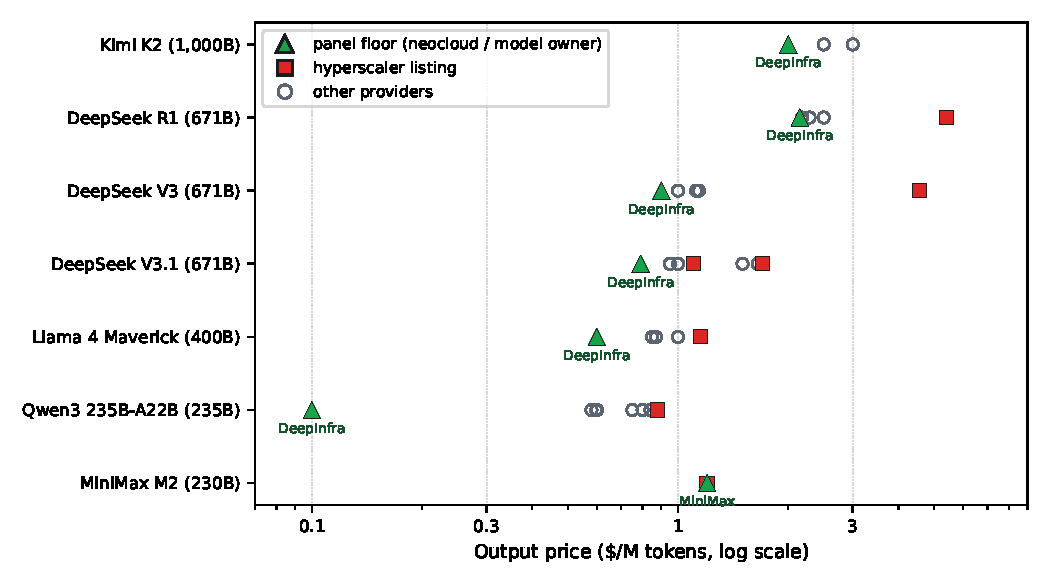
\includegraphics[width=\linewidth]{fig3_floors.pdf}
\caption{The figure plots every provider's output price for the seventeen
primary-panel models of 200B+ total parameters (log scale). The lowest
quote in each panel (filled triangle, labeled) is posted by a neocloud in
eleven panels and by the model's owner in six. Hyperscaler listings
(squares) never set a floor, and the remaining providers (open circles)
fill the range between.}
\label{fig:floors}
\end{figure}

\emph{(b) Hyperscalers price above the floor and never set it.} Hyperscaler
listings appear in five of the seventeen panels (Google Vertex and Amazon
Bedrock; Microsoft Azure lists no open-weight endpoint on the marketplace at
the snapshot date). Their premiums over the panel floor are 1.5$\times$ on
GLM 5 (Bedrock), 1.9$\times$ on Llama 4 Maverick, 1.3$\times$ on GLM 4.7,
1.2$\times$ on MiniMax M2, and 8.8$\times$ on Qwen3-235B-A22B (all Google).
All are positioned as managed enterprise offerings~\cite{r13,r25}.

\emph{(c) Participation no longer declines with footprint.} Here the 2026
market departs from the scale-gating prediction. The trillion-parameter
panels attract some of the largest provider counts in the data (Kimi K2.6,
$n = 20$; GLM 5.2, $n = 22$), while the smallest dense models attract three
to five. Serving a 744B--1{,}000B MoE is no longer the preserve of a few
operators. The timing is consistent with the diffusion mechanism documented
in \S\ref{sec:deepseek}: the expert-parallel serving recipes that were
proprietary craft in early 2025 are now published and reproduced, and
open-source serving stacks have matured around them~\cite{r8,r10}. The
scale barrier H2 posits has not disappeared, but its observable signature
has moved from participation counts to who sets the floor, and to the
dispersion structure below.

\subsection{Secondary result: price dispersion is compressed by selection}
\label{sec:dispersion}

Within-model price dispersion remains compressed for MoE panels: the median
coefficient of variation of output price is 0.23 for the 28 MoE panels
against 0.35 for the 10 dense panels (Figure~\ref{fig:disp}). The rank
correlation between a panel's expert-to-activation ratio $E/k$ and its
dispersion is negative but weaker than the floor result
(Spearman $\rho = -0.24$ over the 37 panels with published $E/k$). The
selection reading is unchanged in kind~\cite{r28,r29}: providers whose
latent cost exceeds the competitive price tend not to list, so the observed
prices of the most scale-demanding models are a truncated sample. The broadened participation
of \S\ref{sec:h2result}(c) weakens the truncation, which is consistent with
the weaker correlation in this snapshot.

\begin{figure}[t]
\centering
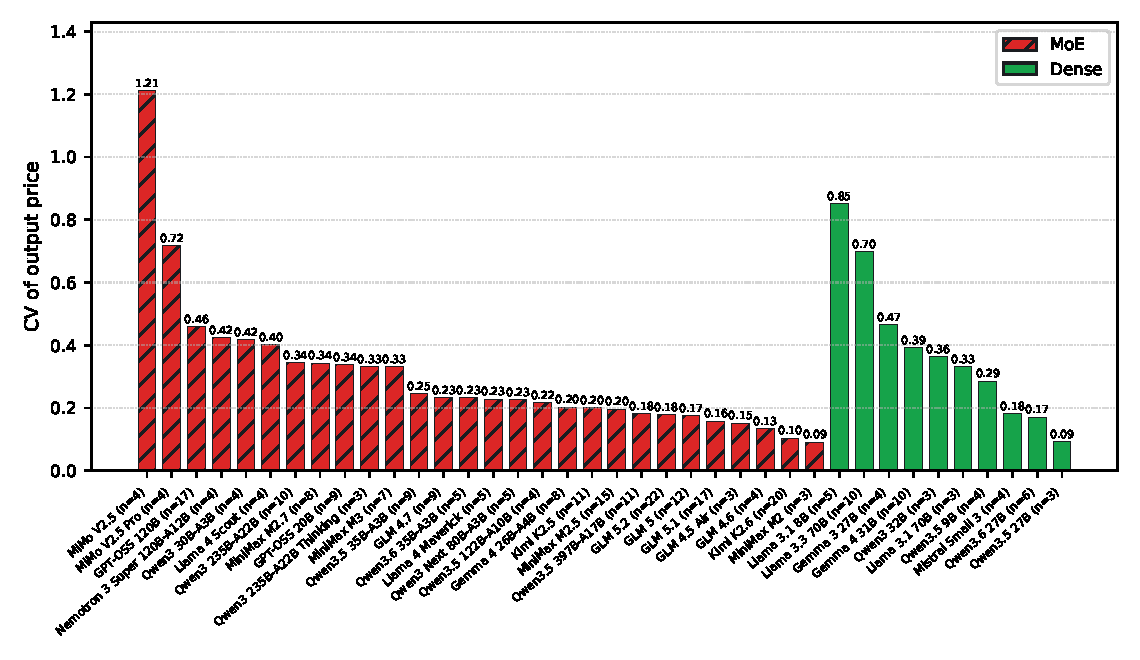
\includegraphics[width=\linewidth]{fig2_dispersion.pdf}
\caption{The figure shows within-model price dispersion, measured as the
coefficient of variation of output price across providers, for MoE panels
(hatched bars) versus dense panels (solid bars) in the primary panel.}
\label{fig:disp}
\end{figure}

\section{The DeepSeek exception}
\label{sec:deepseek}

DeepSeek is excluded from the primary panel because its prices are set by a
different process, and evaluating its panels against the schedule estimated
without them shows exactly what that process does
(Table~\ref{tab:deepseek}). Three regularities stand out.

\begin{table}[t]
\centering
\caption{The table evaluates the seven DeepSeek panels against the primary
schedule of Table~\ref{tab:ols}. ``Schedule'' is the price the ex-DeepSeek
regression predicts for the model's architecture; ``ratio'' is the observed
median over that prediction.}
\label{tab:deepseek}
\small
\begin{tabular}{lrrrlr}
\toprule
Panel & Med \$/M & Schedule & Ratio & Floor setter & $n$ \\
\midrule
DeepSeek R1 (671/37)          & 2.18 & 2.24 & 0.97 & DeepInfra (\$2.15) & 3  \\
DeepSeek V4 Pro (1{,}600/49)  & 3.14 & 3.49 & 0.90 & DeepSeek (\$0.87)  & 13 \\
DeepSeek V3.1 (671/37)        & 1.25 & 2.24 & 0.56 & DeepInfra (\$0.79) & 6  \\
DeepSeek V3 (671/37)          & 1.06 & 2.24 & 0.47 & DeepInfra (\$0.90) & 4  \\
DeepSeek V3.1 Terminus (671/37) & 0.98 & 2.24 & 0.44 & DeepInfra (\$0.95) & 4 \\
DeepSeek V3.2 (671/37)        & 0.45 & 2.24 & 0.20 & StreamLake (\$0.34) & 12 \\
DeepSeek V3.2-Exp (671/37)    & 0.41 & 2.24 & 0.18 & Novita (\$0.41)    & 3  \\
DeepSeek V4 Flash (284/13)    & 0.28 & 1.35 & 0.21 & DeepInfra (\$0.18) & 13 \\
\bottomrule
\end{tabular}
\end{table}

First, the discount is generation-specific, which identifies it as
technological rather than purely strategic. The pre-V3.2 models price near
or moderately below the schedule (R1 at 0.97$\times$, the V3.1 family at
0.44--0.56$\times$), while every model carrying DeepSeek's sparse attention
(V3.2, V3.2-Exp, V4 Flash) is served at roughly one fifth of the schedule
price by a dozen competing third parties. The architecture genuinely lowers
serving cost, and because DeepSeek publishes the serving
recipes~\cite{r10,r8}, third parties can realize the saving and compete it
into prices. The floor setters are the same class of provider that documents
large-scale expert parallelism publicly~\cite{r14}.

Second, the vendor anchors. On its flagship V4 Pro, DeepSeek itself sets the
floor at \$0.87 against a third-party median of \$3.14, underpricing the
competitive market for its own model by 3.6$\times$. This is the
vertical-integration mechanism of H2 in its purest observed form: the one
operator with hyperscale expert-parallel pools for a model prices it where
no third party can follow.

Third, the exception clarifies rather than threatens the footprint result.
Including the DeepSeek panels barely moves the elasticity ratio (0.85
against 0.84), because the schedule is identified from the cross-section of
architectures, not from any one family's level. What DeepSeek breaks is the
fit, not the slope: its sparse-attention generation shows that the cost
frontier itself is moving, and that a vendor with the right strategy can
detach its prices from the market schedule. A popular comparison from the
snapshot week illustrates the point: DeepSeek V4 Flash (284B total) is
served at a lower per-token price than Qwen3.6 35B-A3B (36B total), a
model an eighth its size. Under any parameter-based schedule, including
compute pricing, the larger model should cost more. The inversion is the
combination of a genuine cost technology, published recipes, an owner
anchor, and a launch premium on the smaller model, and it is visible only
because both effects are large.

\section{Discussion and limitations}

Our evidence is observational and market-level: we observe posted prices and
public listings, not provider costs, contracts, or deployments. Five
limitations qualify the interpretation of the results. For each, we state the
limitation and the reason we believe the conclusions survive it.

\begin{itemize}
\item \textbf{Price is not cost.} List prices embed margins, loss-leader
strategies, and enterprise positioning. The footprint elasticity establishes what the market \emph{charges}; the inference to underlying cost is an interpretation. That interpretation is supported by the deployment-cost evidence of Table~\ref{tab:deploy} (EP-pool cost \$0.20--0.50/M against large-MoE floors of \$0.28--3.20) and by the competitive structure of open-weight serving. LMSYS's \$0.20/M and DeepSeek's 545\% margin figures, however, are self-reported, not audited.
\item \textbf{Inference from prices is indirect.} Provider opacity is the
premise of our design (\S1), but it also limits what we can claim. That the
floor-setting neoclouds run large-scale expert parallelism is inferred from
their economics and from the public availability of EP serving software, not
observed; only SiliconFlow documents an EP deployment~\cite{r14}. No small provider
states publicly why it declines to serve 671B-class models; the exit mechanism
rests on documented economics rather than testimony. Our conclusions are
consistency checks of the price structure against publicly reconstructable
cost floors, not observations of provider internals.
\item \textbf{Demand and quality are unobserved.} DeepSeek R1 commands
2.1$\times$ the price of its architecture-identical sibling V3, a
reasoning-model demand premium that the regression absorbs as noise.
Popularity may also correlate with aggressive pricing.
\item \textbf{The panel is a single snapshot.} It reflects one collection
date (2026-07-06) in a market that reprices within weeks, and the residual
structure shows time is not ignorable: newly released models list above the
schedule and DeepSeek's newest generation lists far below it. The collection
pipeline is automated and mechanical, and we intend to re-collect monthly so
that the schedule's stability, and the decay of launch premia, can be
estimated longitudinally.
\item \textbf{The sample has limits.} OpenRouter covers the competitive
open-weight market; hyperscaler-exclusive and closed models are
underrepresented. The
dense subsample is small ($n = 10$) and confined to $\leq$73B, because larger
dense models have left the market, which is itself evidence of footprint
economics. Delivered throughput tiers are not controlled. Finally, capacity
and bandwidth requirements both scale with total parameters, so our test
cannot distinguish ``priced by bytes held'' from ``priced by bytes streamed'';
under either reading, the priced quantity is memory, not compute.
\end{itemize}

\section{Conclusion: implications for inference hardware}

Two results emerge from the serving market's own prices. First, the industry's
original claim for sparsity, that an MoE model costs what its active compute
costs~\cite{r30,r31,r32}, is rejected: the market bills Mixture-of-Experts
models by the memory they occupy, not the compute they perform. The sparsity
elasticity of price is 84\% of the active-parameter elasticity
($p = 1.9 \times 10^{-5}$), so a customer of a 1{,}000B/32B model pays
approximately as if for a $\sim$580B dense model. Second, the price floor
of every large-MoE panel belongs to a vertically integrated provider, a
neocloud or the model's own vendor, and general-purpose clouds price
1.2--8.8$\times$ above the floor and never set it. Participation in
large-MoE serving has broadened as published expert-parallel recipes
diffused, and DeepSeek's sparse-attention generation shows the cost frontier
itself moving; the scale advantage now shows in who sets the floor rather
than in who can serve at all.

Both results point to the same hardware mismatch. The mainstream GPU bundles
enormous compute with scarce, expensive HBM; MoE decoding uses the memory
fully and the compute hardly at all, except inside hyperscale expert-parallel
pools that only a few operators can build. For everyone else, the economically rational serving device is the opposite shape. It has \textbf{large, cheap memory capacity} to hold the full expert set without buying stranded FLOPS. It has \textbf{modest compute}, since decoding at realistic concurrency cannot exercise more. And it has \textbf{moderate bandwidth}, sufficient for interactive token rates and procurable from commodity supply chains rather than the allocation-constrained HBM market. Shipping products are beginning to approximate this design point, notably Apple's Mac Studio (up to 512 GB unified LPDDR5)~\cite{r42}. NVIDIA's DGX Spark (128 GB LPDDR5X)~\cite{r43} supplies the memory capacity but pairs it with a compute-to-bandwidth balance that only datacenter-scale concurrency could exercise, so it meets the capacity criterion alone. Purpose-built decode accelerators instantiate the full design point directly, such as the Skymizer HTX-301, a 28 nm PCIe card carrying 384 GB of commodity LPDDR, whose performance figures are vendor-claimed pending independent benchmarks~\cite{r44}. The
market prices measured here quantify the opportunity such hardware
addresses. The gap between footprint-cheap serving cost and market price is
widest for the most sparse frontier models (the Qwen 35B-A3B generations,
Kimi K2.6, GLM 5.x), which is where the industry is heading.

\paragraph{Data and reproducibility.}
The raw data and analysis code are available at
\url{https://github.com/juntao/memory_is_the_price}. The repository
archives the price snapshot (\path{pd_prices_20260706.json}, 532 raw
endpoint rows for 129 candidate models) and the verified architecture data
(\path{pd_arch_20260706.json}). The analysis script (\path{analysis.py})
is dependency-free Python: OLS via normal equations, exact $t$ and $F$
$p$-values via the incomplete beta function, and Spearman by ranks; the
figures are generated by \path{make_figures.py}. Running \path{analysis.py}
reproduces every statistic in \S4--\S5. All references below were verified by direct fetch at the
time of writing; architecture parameters were verified against each
repository's \path{config.json}.

\begin{thebibliography}{99}
\bibitem{r15} DeepSeek-AI. DeepSeek-V3 technical report. arXiv:2412.19437.
\url{https://arxiv.org/abs/2412.19437}
\bibitem{hf_scout} Meta. Llama-4-Scout-17B-16E-Instruct model repository
($E{=}16$, $k{=}1$). HuggingFace, fetched 2026-07-06.
\url{https://huggingface.co/meta-llama/Llama-4-Scout-17B-16E-Instruct}
\bibitem{hf_maverick} Meta. Llama-4-Maverick-17B-128E-Instruct model
repository ($E{=}128$, $k{=}1$). HuggingFace, fetched 2026-07-06.
\url{https://huggingface.co/meta-llama/Llama-4-Maverick-17B-128E-Instruct}
\bibitem{hf_qwen} Qwen Team. Qwen3-235B-A22B-Instruct-2507 model repository,
\path{config.json} ($E{=}128$, $k{=}8$). HuggingFace, fetched 2026-07-06.
\url{https://huggingface.co/Qwen/Qwen3-235B-A22B-Instruct-2507/raw/main/config.json}
\bibitem{hf_kimi} Moonshot AI. Kimi-K2-Instruct model repository,
\path{config.json} ($E{=}384$, $k{=}8$). HuggingFace, fetched 2026-07-06.
\url{https://huggingface.co/moonshotai/Kimi-K2-Instruct/raw/main/config.json}
\bibitem{hf_oss} OpenAI. gpt-oss-120b model repository, \path{config.json}
($E{=}128$, $k{=}4$). HuggingFace, fetched 2026-07-06.
\url{https://huggingface.co/openai/gpt-oss-120b/raw/main/config.json}
\bibitem{hf_glm} Z.ai. GLM-4.5 model repository, \path{config.json}
(\path{n_routed_experts=160}, $k{=}8$). HuggingFace, fetched 2026-07-06.
\url{https://huggingface.co/zai-org/GLM-4.5/raw/main/config.json}
\bibitem{hf_minimax} MiniMax AI. MiniMax-M2 model repository ($E{=}256$,
$k{=}8$; 230B total / 10B active). HuggingFace, fetched 2026-07-06.
\url{https://huggingface.co/MiniMaxAI/MiniMax-M2}
\bibitem{r30} Fedus, W., Zoph, B., \& Shazeer, N. Switch Transformers:
scaling to trillion parameter models with simple and efficient sparsity.
arXiv:2101.03961, 2021. \url{https://arxiv.org/abs/2101.03961} (``with outrageous numbers of parameters'' at ``a constant computational cost'').
\bibitem{r31} Mistral AI. Mixtral of experts. 2023-12-11.
\url{https://mistral.ai/news/mixtral-of-experts/} (``Mixtral has 46.7B total
parameters but only uses 12.9B parameters per token. It, therefore, processes
input and generates output at the same speed and for the same cost as a 12.9B
model.'')
\bibitem{r32} Databricks. Introducing DBRX: a new state-of-the-art open LLM.
2024-03-27.
\url{https://www.databricks.com/blog/introducing-dbrx-new-state-art-open-llm}
(DBRX inference throughput is ``up to 2x faster'' than Llama2-70B ``thanks to having about half as many active parameters'').
\bibitem{r12} DeepInfra. Series B announcement and DeepCluster owned-hardware
pricing. \url{https://deepinfra.com/blog/deepinfra-series-b};
\url{https://deepinfra.com/deepcluster}
\bibitem{r13} Microsoft Azure AI Foundry, DeepSeek model pricing.
\url{https://azure.microsoft.com/en-us/pricing/details/ai-foundry-models/deepseek/};
Amazon Web Services, DeepSeek-R1 on Bedrock.
\url{https://aws.amazon.com/blogs/aws/deepseek-r1-now-available-as-a-fully-managed-serverless-model-in-amazon-bedrock/}
\bibitem{r25} Google. Llama 4 models generally available as managed API
service on Vertex AI. Google Developers Blog, 2025-04-29.
\url{https://developers.googleblog.com/en/llama-4-ga-maas-vertex-ai/} (``The
underlying infrastructure, scaling, and management costs are incorporated into
the API usage price.''). See also AWS Bedrock model card for DeepSeek-R1
(commercial terms only):
\url{https://docs.aws.amazon.com/bedrock/latest/userguide/model-card-deepseek-deepseek-r1.html}
\bibitem{r1} OpenRouter. Public endpoints API, per-model provider listings.
\url{https://openrouter.ai/api/v1/models/deepseek/deepseek-r1-0528/endpoints}
(pattern identical for all 18 models). Accessed 2026-07-01; re-verified at
writing.
\bibitem{r23} Gao, I., Liang, P., \& Guestrin, C. Model equality testing:
which model is this API serving? ICLR 2025. arXiv:2410.20247.
\url{https://arxiv.org/abs/2410.20247}
\bibitem{r10} DeepSeek-AI. DeepSeek-V3/R1 inference system overview (Open
Infra Index, Day 6).
\url{https://github.com/deepseek-ai/open-infra-index/blob/main/202502OpenSourceWeek/day_6_one_more_thing_deepseekV3R1_inference_system_overview.md}
\bibitem{r8} LMSYS. Deploying DeepSeek with PD disaggregation and large-scale
expert parallelism on 96 H100 GPUs.
\url{https://www.lmsys.org/blog/2025-05-05-large-scale-ep/}
\bibitem{r19} Cloudflare. Serving very large models on Workers AI (Infire;
disaggregated prefill and expert parallelism).
\url{https://blog.cloudflare.com/workers-ai-large-models/}; model catalog:
\url{https://developers.cloudflare.com/workers-ai/models/}
\bibitem{r26} Hayek, F.~A. The use of knowledge in society. \emph{American
Economic Review} 35(4), 519--530, 1945.
\bibitem{r27} Rosen, S. Hedonic prices and implicit markets: product
differentiation in pure competition. \emph{Journal of Political Economy}
82(1), 34--55, 1974.
\bibitem{r24} Erdil, E. Inference economics of language models. Epoch AI.
arXiv:2506.04645, June 2025. \url{https://arxiv.org/abs/2506.04645}. Bottom-up
cost model over arithmetic, memory-bandwidth, network, and latency
constraints; no market-price analysis.
\bibitem{r7} Tensor Economics. MoE inference economics from first principles.
\url{https://www.tensoreconomics.com/p/moe-inference-economics-from-first}
\bibitem{r22} Li, H., et al. When is the same model not the same service? A
measurement study of hosted open-weight LLM APIs. arXiv:2605.02821, May 2026.
\url{https://arxiv.org/abs/2605.02821}. \S4.4 (``Parameter Scale Is Not a
Sufficient Price Model'') raises the active-vs-total pricing question
descriptively.
\bibitem{r21} Scher, A. Observations about LLM inference pricing. MIRI
Technical Governance Team blog, 2025-03-03.
\url{https://techgov.intelligence.org/blog/observations-about-llm-inference-pricing}.
Fits dense price--parameter regressions and compares five MoE models against
the dense trendline.
\bibitem{r4} TrendForce. HBM3e pricing and DDR5 premium.
\url{https://www.trendforce.com/presscenter/news/20251029-12758.html}
\bibitem{r5} Silicon Analysts. AI accelerator cost bridge: HBM share of
manufacturing cost. \url{https://siliconanalysts.com/tools/cost-bridge}
\bibitem{r6} TechSpot. SK hynix sells out semiconductor supply into 2026.
\url{https://www.techspot.com/news/110058-sk-hynix-completely-sells-out-semiconductor-supply-ai.html}
\bibitem{r17} HPC-AI Tech. DeepSeek R1 671B deployment guide (8$\times$H200
reference configuration).
\url{https://company.hpc-ai.com/blog/deepseek-r1-671b-deployment-how-to-maximize-performance}
\bibitem{r9} dzhsurf. DeepSeek V3/R1 deployment benchmarks, 8$\times$H100 (AWQ
4-bit, vLLM).
\url{https://github.com/dzhsurf/deepseek-v3-r1-deploy-and-benchmarks}
\bibitem{r16} DeepSeek-AI. DeepGEMM: grouped GEMM kernels
(BLOCK\_M = 128). \url{https://github.com/deepseek-ai/DeepGEMM}
\bibitem{r33} Patel, P., Choukse, E., et al.\ (Microsoft Azure Research).
Splitwise: efficient generative LLM inference using phase splitting.
arXiv:2311.18677, 2023. \url{https://arxiv.org/abs/2311.18677}
\bibitem{r34} Zhong, Y., et al. DistServe: disaggregating prefill and decoding
for goodput-optimized large language model serving. OSDI 2024.
arXiv:2401.09670. \url{https://arxiv.org/abs/2401.09670}
\bibitem{r35} Qin, R., et al.\ (Moonshot AI). Mooncake: a KVCache-centric
disaggregated architecture for LLM serving. arXiv:2407.00079, 2024.
\url{https://arxiv.org/abs/2407.00079}
\bibitem{r11} NVIDIA. Scaling large MoE models with wide expert parallelism on
NVL72 rack-scale systems.
\url{https://developer.nvidia.com/blog/scaling-large-moe-models-with-wide-expert-parallelism-on-nvl72-rack-scale-systems/}
\bibitem{r2} Artificial Analysis. Provider comparison pages.
\url{https://artificialanalysis.ai/models/deepseek-r1/providers}
\bibitem{hf_r1} DeepSeek-AI. DeepSeek-R1-0528 model repository,
\path{config.json} ($E{=}256$, $k{=}8$). HuggingFace, fetched 2026-07-06.
\url{https://huggingface.co/deepseek-ai/DeepSeek-R1-0528/raw/main/config.json}
\bibitem{r18} DeepInfra. Qwen3-235B-A22B-Instruct-2507 price page
(loss-leader verification).
\url{https://deepinfra.com/Qwen/Qwen3-235B-A22B-Instruct-2507}
\bibitem{r28} Stigler, G.~J. The economics of information. \emph{Journal of
Political Economy} 69(3), 213--225, 1961.
\bibitem{r29} Heckman, J.~J. Sample selection bias as a specification error.
\emph{Econometrica} 47(1), 153--161, 1979.
\bibitem{r14} Huawei \& SiliconFlow. Serving large language models on Huawei
CloudMatrix384. arXiv:2506.12708. \url{https://arxiv.org/pdf/2506.12708}
\bibitem{r42} Apple. Apple reveals M3 Ultra, taking Apple silicon to a new
extreme. Newsroom, March 2025.
\url{https://www.apple.com/newsroom/2025/03/apple-reveals-m3-ultra-taking-apple-silicon-to-a-new-extreme/}
\bibitem{r43} NVIDIA. DGX Spark.
\url{https://www.nvidia.com/en-us/products/workstations/dgx-spark/}
\bibitem{r44} Skymizer Taiwan Inc. HTX-301 announcement (April 2026) and
company profile v1.0 (March 2026). Performance figures vendor-claimed and
pre-production.
\end{thebibliography}

\end{document}
